% Polished version of Chen's method draft (his red text, with the black text inside his sections), 23 Sep 2026.
% Structure and terminology follow his version 2; wording tightened, placeholders filled where the bib has the reference.
% Labels kept identical to the current section so every cross-reference in the paper still resolves.
\begin{figure}[!htb]
\centering
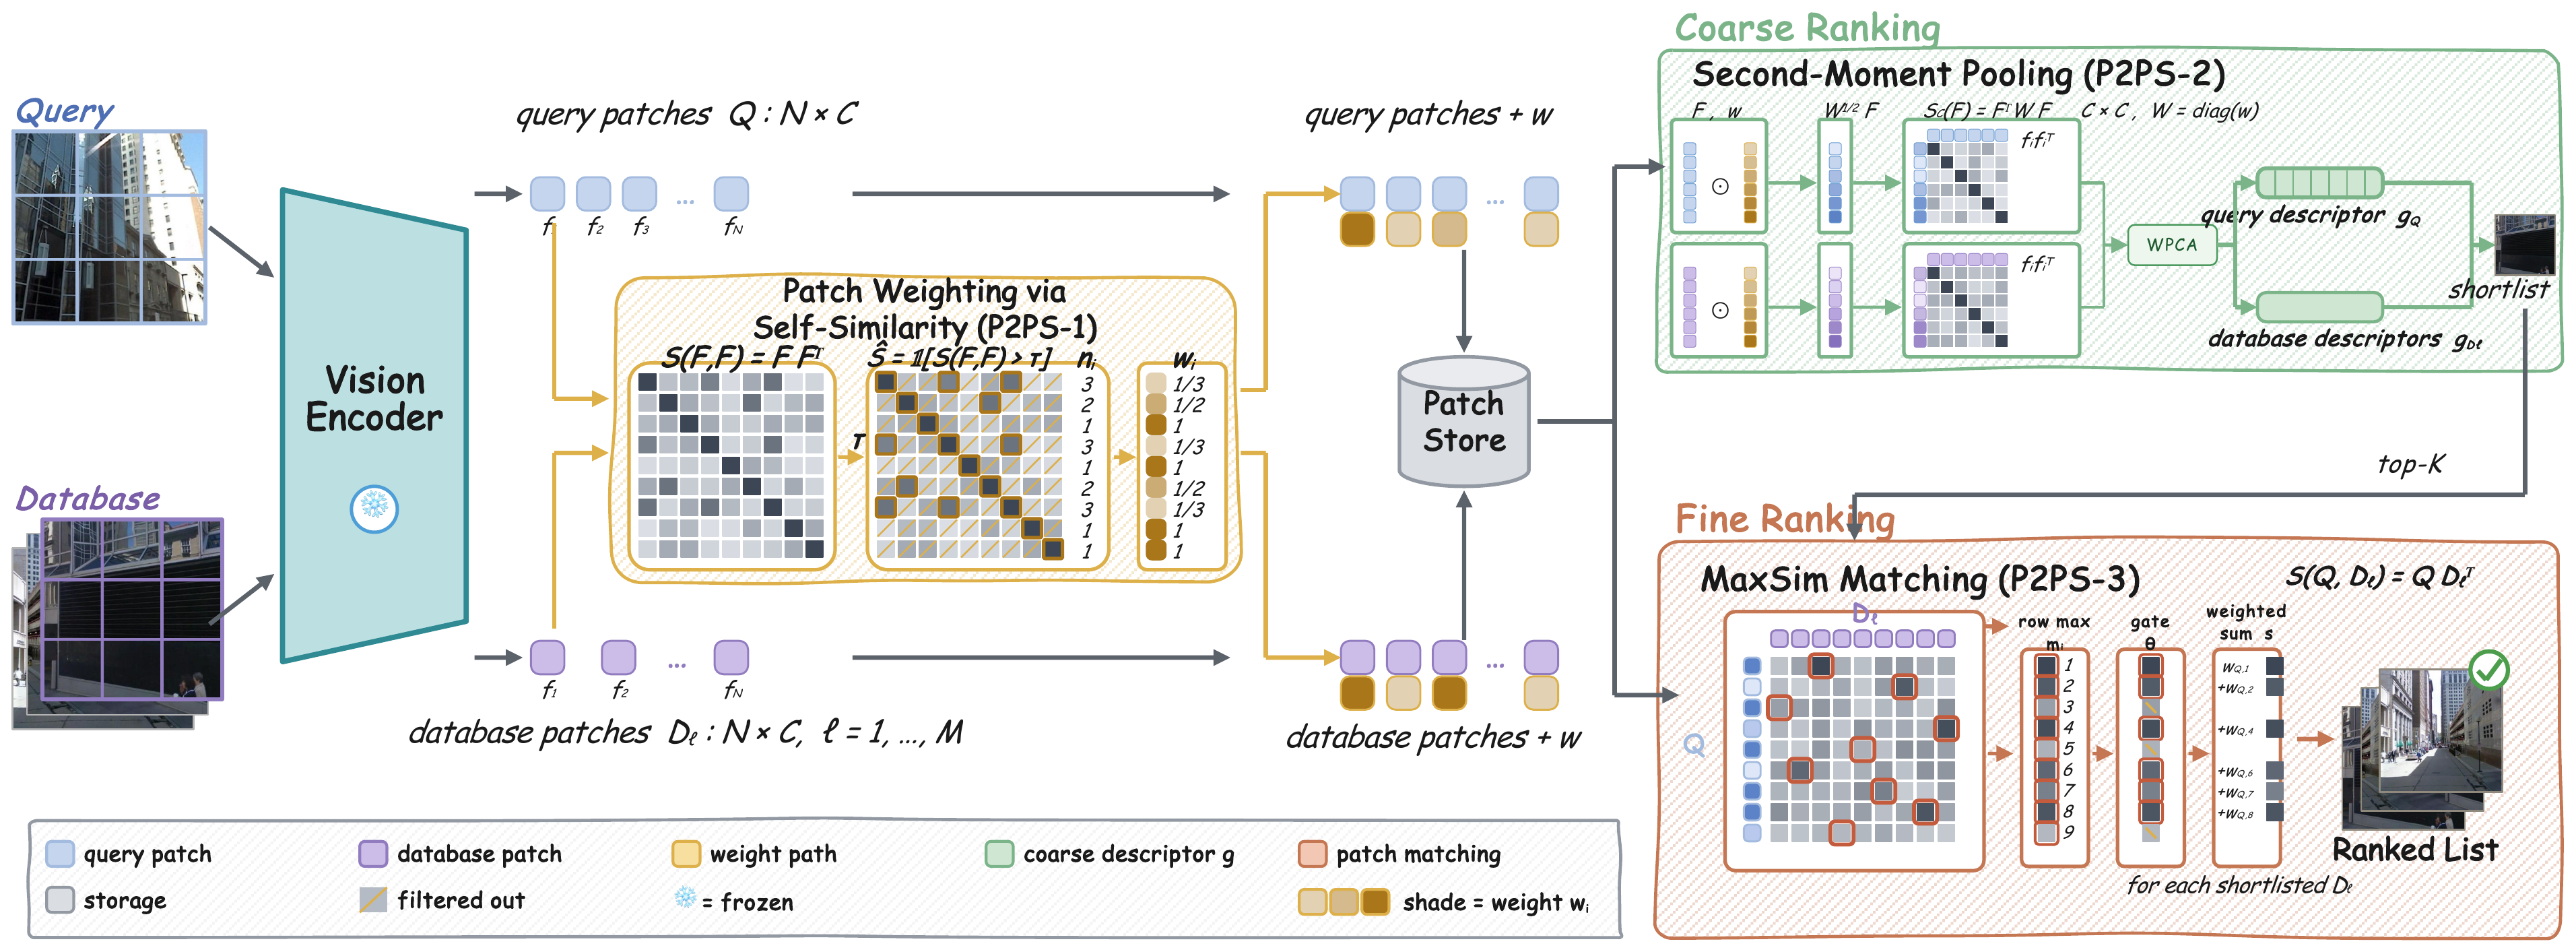
\includegraphics[width=0.92\textwidth]{figures/method_fig_ppt.png}
\caption{\textbf{Overview of the proposed method.} Each image is partitioned into patches and encoded once by a frozen backbone. One patch-to-patch similarity (P2PS) template $S(A,B)=AB^{\top}$ is read three times: within an image it yields the patch weights $w_i{=}1/n_i$ (P2PS-1); between a query and the database it is pooled into one second-order descriptor per image for coarse ranking (P2PS-2), and read row by row as \textsc{MaxSim} matching for fine ranking of the shortlist (P2PS-3).}
\label{fig:method}
\end{figure}

\section{Method}
\label{sec:method}
As illustrated in Figure~\ref{fig:method}, the proposed method follows a training-free paradigm: it requires neither model training nor annotated data. Every step of the pipeline relies on a single patch-to-patch similarity (P2PS) template, read in three different forms. The query and the database images are first partitioned into patches, whose features are extracted by a frozen pretrained vision model. Each image then computes the similarity between its own patches (P2PS-1), from which a weight for every patch is derived (\S\ref{sec:feat}). Retrieval proceeds in a coarse-to-fine manner (\S\ref{sec:coarse_to_fine_ranking}): second-order pooling of the weighted patch features gives one compact descriptor per image, with which the whole database is ranked (P2PS-2), and patch-to-patch \textsc{MaxSim} matching between the query and the top-ranked candidates refines that ranking (P2PS-3). The three forms are summarized in Table~\ref{tab:readings} and detailed below.
\begin{center}
\footnotesize\setlength{\tabcolsep}{5pt}\renewcommand{\arraystretch}{1.05}
\resizebox{\linewidth}{!}{%
\begin{tabular}{lllcl}
\toprule
 & Form of $S(A,B)$ & Formula & Needs the pair & Used for \\
\midrule
P2PS-1 & $S(F,F)$, count per row above $\tau$ & $w_i=1\big/\sum_j \mathbb 1[S(F,F)_{ij}>\tau]$ & no & patch weighting (\S\ref{sec:feat}) \\
P2PS-2 & $S(Q,D)$, weighted sum of squares & $\sum_{i,j} w_{Q,i}w_{D,j}S(Q,D)_{ij}^2=\langle G_C(Q),G_C(D)\rangle$ & no & coarse ranking of $\mathcal D$ (\S\ref{sec:coarse_to_fine_ranking}) \\
P2PS-3 & $S(Q,D)$, weighted row maxima & $s(Q,D)=\sum_i w_{Q,i}\,\mathbb 1[m_i>\theta]\,m_i$ & yes & fine ranking of the top-$K$ (\S\ref{sec:coarse_to_fine_ranking}) \\
\bottomrule
\end{tabular}}
\captionof{table}{The three forms of the P2PS template. ``Needs the pair'' marks the form that cannot be precomputed per image.}
\label{tab:readings}
\end{center}

\subsection{Problem Formulation and Notation}
\label{sec:prelim}
Given a query image $I_q$ and a database $\mathcal{D}=\{(I_d,\mathbf c_d)\}$ of images $I_d$ with known spatial coordinates $\mathbf c_d$, visual place recognition retrieves the database image that best matches the query and returns its coordinates as the estimate $\hat{\mathbf c}_q$ \citep{netvlad}. As discussed in \S\ref{sec:related}, most existing solutions train a dedicated model on a large annotated corpus $\mathcal{D}^{T}=\{(I_t,\mathbf c_t)\}$ for this retrieval, and the model has to be trained again whenever the backbone changes.

The proposed method removes this requirement. As shown in Figure~\ref{fig:method}, every image $I$, whether the query or a database image, is partitioned into $N$ patches, $I=[\,p_1,\dots,p_N\,]$, and passed once through a frozen DINOv2/DINOv3 backbone, from which we keep the value facet of one block, the output of its value projection \citep{vitfacets,effovpr}. A PCA fitted on unlabelled database tokens reduces every patch feature to $C{=}512$ channels, and the features are $\ell_2$-normalized. Each image is therefore represented by a patch feature matrix $F=[\,\mathbf f_1,\dots,\mathbf f_N\,]^{\top}\in\mathbb R^{N\times C}$; we write $Q$ for the query and $D_m$ for the $m$-th database image, $m=1,\dots,M$. All computations below use one template, the patch-to-patch similarity
\begin{equation}\label{eq:p2ps}
  S(A,B)=AB^{\top},\qquad S(A,B)_{ij}=\mathbf a_i^{\top}\mathbf b_j,
\end{equation}
the cosine between patch $i$ of $A$ and patch $j$ of $B$. Setting $A$ and $B$ to different feature matrices gives the three forms of Table~\ref{tab:readings}: $A{=}B{=}F$ for patch weighting, and $A{=}Q$, $B{=}D_m$ for coarse and fine ranking. Supplementary~\S\ref{app:hyper} sweeps the block, the facet and the shortlist depth.

\subsection{Patch Weighting via Self-Similarity (P2PS-1)}
\label{sec:feat}
When two images of the same place are compared patch by patch, not every patch is equally informative. Sky, pavement and a facade of identical windows fill an image with near-copies of the same content; ten nearly identical sky patches should contribute about as much as one distinctive patch, not ten times as much. We therefore assign each patch a weight that decreases with the number of near-copies it has within its own image.

The P2PS template with $A{=}B{=}F$ gives the Gram matrix $G=S(F,F)=FF^{\top}\in\mathbb R^{N\times N}$, whose entry $G_{ij}$ is the similarity between patches $p_i$ and $p_j$ of the same image. We binarize it with a similarity threshold $\tau$,
\begin{equation}\label{eq:demo}
  \hat G_{ij}=\mathbb 1\left[\,G_{ij}>\tau\,\right],
\end{equation}
where $\mathbb 1[\cdot]$ is the indicator function, so that $\hat G$ counts near-copies rather than grading them. The weight of patch $p_i$ is the reciprocal of its number of near-copies,
\begin{equation}\label{eq:weight}
  w_i=\frac{1}{n_i},
  \qquad
  n_i=\sum_{j=1}^{N}\hat G_{ij},
\end{equation}
where $n_i$ counts the patches, including $p_i$ itself, that are highly similar to $p_i$, that is, the nonzero entries in row $i$ of $\hat G$ (Figure~\ref{fig:method}). A patch that recurs across the image has a large $n_i$ and receives a small weight; a distinctive patch with few or no near-copies receives a large weight, up to $w_i{=}1$. This rule is the closed-form solution of the democratic-weighting condition $\hat G\mathbf w=\mathbf 1$ of \citet{democratic} and \citet{gmp} when repeated content forms blocks of mutual near-duplicates (Supplementary~\S\ref{app:ridge}); on real images the condition holds approximately (Table~\ref{tab:residual}), and what the method relies on, that $w_i$ falls with the amount of similar content around patch $i$, holds regardless (Figure~\ref{fig:blocks}). The weights are used in both ranking stages below.

\begin{figure}[!htb]
\centering
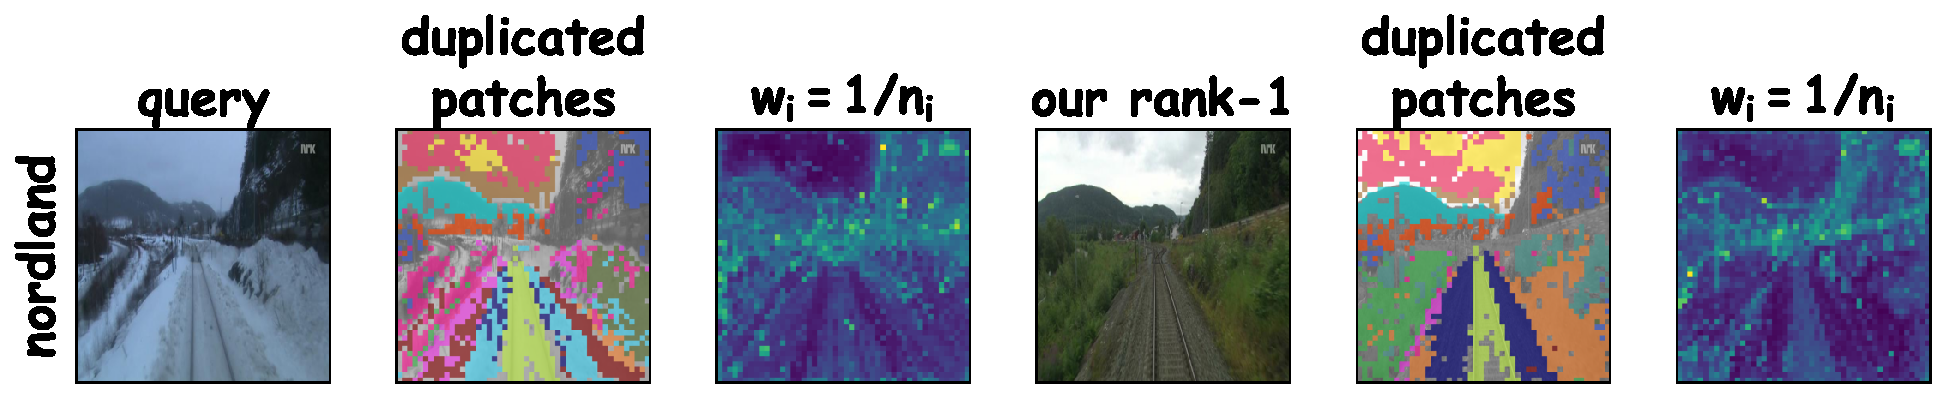
\includegraphics[width=0.78\textwidth]{figures/blocks_nordland.pdf}
\caption{Duplicated patches and their weights on one Nordland pair. Left, the query; right, the database image retrieved at rank one. Colours mark blocks of mutually near-duplicate patches under $\hat G$, grey patches join no block, and the heat maps show $w_i{=}1/n_i$ on a log scale over all $2{,}304$ tokens: snow, sky and the track bed receive little weight, the sparse distinctive content receives most. Every benchmark is shown in Supplementary~\S\ref{app:patchvis}.}
\label{fig:blocks}
\end{figure}

\subsection{Coarse-to-Fine Ranking}
\label{sec:coarse_to_fine_ranking}
Retrieval follows the classical coarse-to-fine pipeline \citep{patchnetvlad,r2former,selavpr}: a compact descriptor ranks the whole database, and a more expensive patch-level comparison refines the top of that ranking. Both steps read the P2PS template between the query and a database image, $S(Q,D_m)$, weighted by \eqref{eq:weight}.

\paragraph{Coarse Ranking (P2PS-2).}
\label{sec:global}
Coarse ranking compares the query with every image of a large database, so it needs one compact descriptor per image. We obtain it by weighted second-order pooling of the patch features. Given $F$ and its weights $\mathbf w=[w_1,\dots,w_N]$, the descriptor is the $C\times C$ weighted second-moment matrix
\begin{equation}\label{eq:gc}
  G_C(F)=\frac{1}{\sum_i w_i}\sum_i w_i\,\mathbf f_i\mathbf f_i^{\top},
\end{equation}
in which distinctive patches contribute more. Its inner product between a query and a database image equals the weighted sum of all squared patch-to-patch similarities,
\begin{equation}\label{eq:so-deriv}
  \big\langle\, G_C(Q),\ G_C(D_m)\,\big\rangle
  =\sum_{i,j} w_{Q,i}\,w_{D_m,j}\,S(Q,D_m)_{ij}^{2},
\end{equation}
because $(\mathbf q^{\top}\mathbf d)^2=\langle\mathbf q\mathbf q^{\top},\mathbf d\mathbf d^{\top}\rangle$ for any two patches. The square is what makes this possible: the same sum over the similarities themselves reduces to an inner product of two weighted mean vectors, which retains far less of the image (Supplementary~\S\ref{app:coarsegrid}); in kernel terms \eqref{eq:so-deriv} is a degree-two polynomial match kernel over patches \citep{smk}, the case that factorizes into per-image descriptors (Supplementary~\S\ref{app:factorize}). As $G_C$ is high-dimensional, we follow common practice for second-order descriptors \citep{bcnn,mpncov} and compress it into a compact vector $\mathbf g=\rho(G_C)$ by flattening, $\ell_2$-normalization and whitened PCA. Denoting the query and database descriptors by $\mathbf g_Q$ and $\mathbf g_{D_m}$, coarse ranking sorts the database by $\mathbf g_Q^{\top}\mathbf g_{D_m}$ and keeps the top-$K$ images for fine ranking.

\paragraph{Fine Ranking (P2PS-3).}
\label{sec:core}
Fine ranking reads $S(Q,D_m)$ row by row for each of the $K$ candidates. For every query patch we find its most similar patch in the candidate and sum these best matches,
\begin{equation}\label{eq:stage2}
  s(Q,D_m)=\sum_{i=1}^{N} w_{Q,i}\;\mathbb 1[\,m_i>\theta\,]\;m_i,
  \qquad
  m_i=\max_{j} S(Q,D_m)_{ij},
\end{equation}
the sum of best matches introduced by chamfer matching for comparing two images \citep{chamfer} and known as \textsc{MaxSim} in late-interaction retrieval \citep{colbert}, here weighted by the same $w_{Q,i}$ as in coarse ranking. Sky, pedestrians and occluders have no counterpart in the other image, so a patch counts only if its best match clears a confidence threshold $\theta$, fixed at $0.65$ for every benchmark (Supplementary~\S\ref{app:calib}). The row maximum keeps track of which patch matched which, and for that reason $s(Q,D_m)$ cannot be written as an inner product of two per-image vectors (Supplementary~\S\ref{app:nofactor}); this is why it is applied only to the shortlist, and why a method that stores a single vector per image has no access to it and must instead train its pooling until that vector separates places on its own \citep{netvlad}. The candidates are re-sorted by $s(Q,D_m)$, and the top one gives the query's location.
